\documentclass[american,man]{apa6}

\usepackage{amssymb,amsmath}
\usepackage{ifxetex,ifluatex}
\usepackage{fixltx2e} % provides \textsubscript
\ifnum 0\ifxetex 1\fi\ifluatex 1\fi=0 % if pdftex
  \usepackage[T1]{fontenc}
  \usepackage[utf8]{inputenc}
\else % if luatex or xelatex
  \ifxetex
    \usepackage{mathspec}
    \usepackage{xltxtra,xunicode}
  \else
    \usepackage{fontspec}
  \fi
  \defaultfontfeatures{Mapping=tex-text,Scale=MatchLowercase}
  \newcommand{\euro}{€}
\fi
% use upquote if available, for straight quotes in verbatim environments
\IfFileExists{upquote.sty}{\usepackage{upquote}}{}
% use microtype if available
\IfFileExists{microtype.sty}{\usepackage{microtype}}{}
\usepackage{color}
\usepackage{fancyvrb}
\newcommand{\VerbBar}{|}
\newcommand{\VERB}{\Verb[commandchars=\\\{\}]}
\DefineVerbatimEnvironment{Highlighting}{Verbatim}{commandchars=\\\{\}}
% Add ',fontsize=\small' for more characters per line
\usepackage{framed}
\definecolor{shadecolor}{RGB}{248,248,248}
\newenvironment{Shaded}{\begin{snugshade}}{\end{snugshade}}
\newcommand{\KeywordTok}[1]{\textcolor[rgb]{0.13,0.29,0.53}{\textbf{{#1}}}}
\newcommand{\DataTypeTok}[1]{\textcolor[rgb]{0.13,0.29,0.53}{{#1}}}
\newcommand{\DecValTok}[1]{\textcolor[rgb]{0.00,0.00,0.81}{{#1}}}
\newcommand{\BaseNTok}[1]{\textcolor[rgb]{0.00,0.00,0.81}{{#1}}}
\newcommand{\FloatTok}[1]{\textcolor[rgb]{0.00,0.00,0.81}{{#1}}}
\newcommand{\CharTok}[1]{\textcolor[rgb]{0.31,0.60,0.02}{{#1}}}
\newcommand{\StringTok}[1]{\textcolor[rgb]{0.31,0.60,0.02}{{#1}}}
\newcommand{\CommentTok}[1]{\textcolor[rgb]{0.56,0.35,0.01}{\textit{{#1}}}}
\newcommand{\OtherTok}[1]{\textcolor[rgb]{0.56,0.35,0.01}{{#1}}}
\newcommand{\AlertTok}[1]{\textcolor[rgb]{0.94,0.16,0.16}{{#1}}}
\newcommand{\FunctionTok}[1]{\textcolor[rgb]{0.00,0.00,0.00}{{#1}}}
\newcommand{\RegionMarkerTok}[1]{{#1}}
\newcommand{\ErrorTok}[1]{\textbf{{#1}}}
\newcommand{\NormalTok}[1]{{#1}}
  \usepackage{graphicx}
  \makeatletter
  \def\maxwidth{\ifdim\Gin@nat@width>\linewidth\linewidth\else\Gin@nat@width\fi}
  \def\maxheight{\ifdim\Gin@nat@height>\textheight\textheight\else\Gin@nat@height\fi}
  \makeatother
  % Scale images if necessary, so that they will not overflow the page
  % margins by default, and it is still possible to overwrite the defaults
  % using explicit options in \includegraphics[width, height, ...]{}
  \setkeys{Gin}{width=\maxwidth,height=\maxheight,keepaspectratio}
\ifxetex
  \usepackage[setpagesize=false, % page size defined by xetex
              unicode=false, % unicode breaks when used with xetex
              xetex]{hyperref}
\else
  \usepackage[unicode=true]{hyperref}
\fi
\hypersetup{breaklinks=true,
            bookmarks=true,
            pdfauthor={Frederik Aust},
            pdftitle={Example manuscript to demonstrate the R2APA markdown template},
            colorlinks=true,
            citecolor=blue,
            urlcolor=blue,
            linkcolor=magenta,
            pdfborder={0 0 0}}
\urlstyle{same}  % don't use monospace font for urls
\setlength{\parindent}{0pt}
\setlength{\parskip}{6pt plus 2pt minus 1pt}
\setlength{\emergencystretch}{3em}  % prevent overfull lines
\setcounter{secnumdepth}{0}
\ifxetex
  \usepackage{polyglossia}
  \setmainlanguage{}
\else
  \usepackage[american]{babel}
\fi

 % Line numbering
  \usepackage{lineno}
  \linenumbers


% Manuscript styling
\captionsetup{font=singlespacing,justification=justified}
\usepackage{csquotes}


% Essential manuscript parts
  \title{Example manuscript to demonstrate the R2APA markdown template}
  \shorttitle{RMarkdown to APA}
  \author{Frederik Aust}
  \affiliation{University of Cologne}
  \note{The R2APA-template and further instructions can be retrieved from
\url{https://github.com/crsh/r2apa}. Hail and praises may be sent to
\href{mailto:frederik.aust@uni-koeln.de}{frederik.aust@uni-koeln.de}.}
  \abstract{This example manuscript demonstrates how to use RStudio and RMarkdown to
produce an APA conform manuscript. Using pandoc this file can be
converted to HTML, LaTeX/PDF, or Word documents. At this point, only PDF
documents conform to the APA mansucript guidelines.}


\begin{document}

\maketitle

As you may have heard, recently, there has been a growing interest in
reproducible research. Reproducible data analysis is an easy to
implement yet important aspect of the strive towards reproducibility.
For users of the scripting language \emph{R}, RMarkdown has been
suggested as one possible framework for reproducible analyses. This
example document assumes you have hoped onto the band wagon and know how
to use RMarkdown to conduct and comment your analyses. If you're new to
RMarkdown I recommend you get to grips with it first.

I use \href{http://www.rstudio.com/}{RStudio} (which makes use of
\href{http://johnmacfarlane.net/pandoc/}{pandoc}) to create my
documents, but the general process should work when using pandoc
directly from the command line. When you click RStudio's \emph{Knit}
button a document will be generated that includes both content as well
as the output of any embedded R code chunks within the document. You can
embed an R code chunk like this:

\begin{Shaded}
\begin{Highlighting}[]
\KeywordTok{summary}\NormalTok{(cars)}
\end{Highlighting}
\end{Shaded}

\begin{verbatim}
##      speed           dist    
##  Min.   : 4.0   Min.   :  2  
##  1st Qu.:12.0   1st Qu.: 26  
##  Median :15.0   Median : 36  
##  Mean   :15.4   Mean   : 43  
##  3rd Qu.:19.0   3rd Qu.: 56  
##  Max.   :25.0   Max.   :120
\end{verbatim}

For prettier tables, I suggest you take a look at the \texttt{xtable}
package (for an example, see last page of this document; as required by
the APA guidelines, the table is printed to the final pages of the
document) although there are other ways of doing this. Unfortunately,
for now, the caption is set to the left page margin. :(

\begin{Shaded}
\begin{Highlighting}[]
\KeywordTok{library}\NormalTok{(xtable)}
\KeywordTok{print}\NormalTok{(}
  \KeywordTok{xtable}\NormalTok{(}\KeywordTok{summary}\NormalTok{(cars), }\DataTypeTok{caption =} \StringTok{"Pretty table produced with the xtable-package."}\NormalTok{)}
  \NormalTok{, }\DataTypeTok{comment =} \OtherTok{FALSE}
  \NormalTok{, }\DataTypeTok{booktabs =} \OtherTok{TRUE}
  \NormalTok{, }\DataTypeTok{caption.placement =} \StringTok{"top"}
  \NormalTok{, }\DataTypeTok{include.rownames =} \OtherTok{FALSE}
\NormalTok{)}
\end{Highlighting}
\end{Shaded}

\begin{table}[ht]
\centering
\caption{Pretty table produced with the xtable-package.} 
\begin{tabular}{ll}
  \toprule
    speed &      dist \\ 
  \midrule
Min.   : 4.0   & Min.   :  2   \\ 
  1st Qu.:12.0   & 1st Qu.: 26   \\ 
  Median :15.0   & Median : 36   \\ 
  Mean   :15.4   & Mean   : 43   \\ 
  3rd Qu.:19.0   & 3rd Qu.: 56   \\ 
  Max.   :25.0   & Max.   :120   \\ 
   \bottomrule
\end{tabular}
\end{table}

You can also embed plots, for example:

\begin{Shaded}
\begin{Highlighting}[]
\KeywordTok{plot}\NormalTok{(cars)}
\end{Highlighting}
\end{Shaded}

\begin{figure}[htbp]
\centering
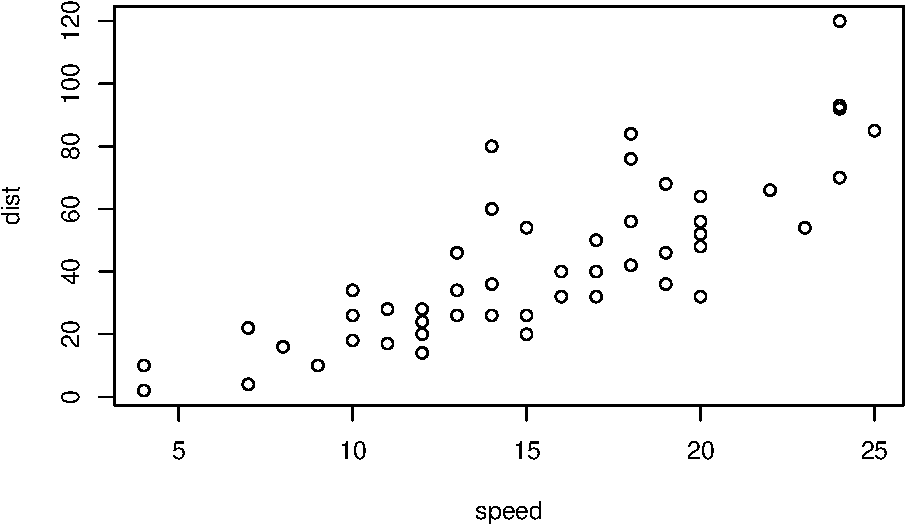
\includegraphics{./example_files/figure-latex/unnamed-chunk-3.pdf}
\caption{Exmple figure created by in-document R code.}
\end{figure}

As required by the APA guidelines, the figure is printed to the final
pages of the document. In RStudio you may have to click the gear (edit
the RMarkdown format options), switch to the tab \enquote{Figures} and
check the option \enquote{Render figures with captions} to make this
work.

The line numbering can be deactivated in the header of this document by
removing the \texttt{lineno} argument.

Finally, you can easily insert citations (e.g., {Baumer},
{Cetinkaya-Rundel}, {Bray}, {Loi}, \& {Horton}, 2014). Citing without
parentheses is, of course, also possible: {Baumer} et al. (2014). The
citation style is set in the header of this document. The relevant
references will, of course, be added to the documents references
automatically.

That's all I have for now. Enjoy writing your manuscript. If you have an
trouble or ideas for improve ments, send me an E-Mail, open an
\href{https://github.com/crsh/r2apa/issues}{issue} on GitHub or make a
pull request with the fix. ;)

\section{References}\label{references}

{Baumer}, B., {Cetinkaya-Rundel}, M., {Bray}, A., {Loi}, L., \&
{Horton}, N. J. (2014). R Markdown: Integrating A Reproducible Analysis
Tool into Introductory Statistics. \emph{ArXiv E-Prints}. Retrieved from
\url{http://adsabs.harvard.edu/abs/2014arXiv1402.1894B}



\end{document}